\documentclass{amsart}
\title[The Lie Hasse package]{The Lie Hasse package \\ Version 1.0}
%% My name:
\makeatletter
\DeclareRobustCommand{\scotsMc}{\scotsMcx{c}}
\DeclareRobustCommand{\scotsMC}{\scotsMcx{\textsc{c}}}
\DeclareRobustCommand{\scotsMcx}[1]{%
  M%
  \raisebox{\dimexpr\fontcharht\font`M-\height}{%
    \check@mathfonts\fontsize{\sf@size}{0}\selectfont
    \kern.3ex\underline{\kern-.3ex #1\kern-.3ex}\kern.3ex
  }%
}
\expandafter\def\expandafter\@uclclist\expandafter{%
  \@uclclist\scotsMc\scotsMC
}
\makeatother
\newcommand{\authorsname}{\texorpdfstring{Benjamin \scotsMc{}Kay}{Benjamin McKay}}
\author{\authorsname}
\address{School of Mathematical Sciences,  University College Cork, Cork, Ireland}
\email{b.mckay@ucc.ie}
\date{3 February 2020}
\usepackage{etex}
\usepackage[T1]{fontenc}
\usepackage[utf8]{inputenx}
\usepackage{etoolbox} 
\usepackage{lmodern}
\RequirePackage[tt=lining]{cfr-lm}
\usepackage[kerning=true,tracking=true]{microtype}
\usepackage{amsmath}
\usepackage{amsfonts}
\usepackage{mathtools}
\usepackage{mathtext}
\usepackage[english]{babel}
\usepackage[pagebackref]{hyperref}
 \hypersetup{
   colorlinks   = true,  %Colours links instead of ugly boxes
   urlcolor     = black, %Colour for external hyperlinks
   linkcolor    = black, %Colour of internal links
   citecolor    = black  %Colour of citations
 }
\usepackage{lie-hasse}
\usetikzlibrary{positioning}
\usepackage{fancyvrb}\fvset{obeytabs,tabsize=2,fontsize=\small}
\usepackage[listings]{tcolorbox} 
\tcbuselibrary{breakable}
\tcbuselibrary{skins}
\usepackage{varwidth}
\usepackage{xspace}
\newcommand{\TikZ}{Ti\textit{k}Z\xspace}
\definecolor{example-color}{gray}{1}
\definecolor{example-border-color}{gray}{.8} 
\tcbset{
	coltitle=black,
	colback=example-color,
	colframe=example-border-color,
	enhanced,breakable,
	pad at break*=1mm,
	toprule=1.2mm,
	bottomrule=1.2mm,
	leftrule=1mm,
	rightrule=1mm,
	toprule at break=-1mm,
	bottomrule at break=-1mm,
	before upper={\widowpenalties=3 10000 10000 150}
}
\tikzset{
	/Dynkin diagram,
	edge length=1cm,
	ordering=Carter,
	vertical shift=0}
\tikzset{
	background rectangle/.style={
		shade,
		top color=olive!20,
		bottom color=white,
		draw=olive!15,
		very thick,
		rounded corners},
}
\begin{document}
\maketitle
\begin{center}%
	\begin{tikzpicture}[show background rectangle]
		\hasse[
			edge/.style={},
			root radius=.02cm,
			edge length=.5cm,
			edge quotes/.style={opacity=0}%
			]{E}{8}%
	\end{tikzpicture}%
\end{center}%
\begin{center}
\begin{varwidth}{\textwidth}
\tableofcontents
\end{varwidth}
\end{center}
\setlength{\arrayrulewidth}{1.5pt}

\section{Quick introduction}
This package draws the Hasse diagram of the poset of the positive simple roots of each complex simple Lie group, as drawn by Ringel \cite{Ringel:2013}.
\begin{tcolorbox}[title={Load the package}]
\begin{Verbatim}
\documentclass{article}
\usepackage{lie-hasse}
\begin{document}
The Hasse diagram of \(F_4\) is 
\begin{center}
\hasse[edge length=1cm]{F}{4}
\end{center}
\end{document}
\end{Verbatim}
\end{tcolorbox}
\par\noindent{}The Hasse diagram of \(F_4\) is 
\begin{center}
\hasse[edge length=1cm]{F}{4}
\end{center}
Each edge is labelled with the simple root by which vertices differ.
\begin{tcblisting}{title={Inside a \TikZ statement}}
\(B_4\) has Dynkin diagram \tikz \dynkin[edge length=.35cm]{B}{4};, Hasse diagram
\begin{center}
\hasse[edge length=1cm]{B}{4}
\end{center}
\end{tcblisting}
\begin{tcblisting}{title={Inside a Dynkin diagram environment, diagrams fit together}}
The Hasse diagram of \(B_4\) is 
\begin{dynkinDiagram}[vertical shift=0,edge length=1cm]{B}{4}
\hasse{B}{4}
\end{dynkinDiagram}
\end{tcblisting}
We shut off the default vertical shift of the Dynkin diagram, so that it starts at the origin.
There is an option to \verb!\hasse! for this:
\begin{tcblisting}{title={Attaching the Dynkin diagram}}
The Hasse diagram of \(B_4\) is 
\begin{center}
\hasse[attach Dynkin diagram=true]{B}{4}
\end{center}
\end{tcblisting}
Unfortunately, attaching a Dynkin diagram looks terrible for \(D\) or \(E\) series, so a Dynkin diagram appears below.
\begin{tcblisting}{title={Attaching the Dynkin diagram}}
The Hasse diagram of \(D_5\) is 
\begin{center}
\hasse[attach Dynkin diagram=true]{D}{5}
\end{center}
\end{tcblisting}
\begin{tcblisting}{title={Inside a \TikZ environment}}
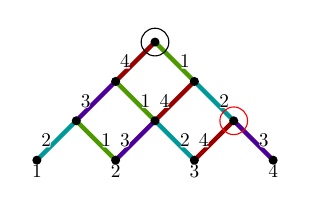
\begin{tikzpicture}
\hasse{A}{4}
\draw (4;1) circle (5pt);
\draw[red] (2;3) circle (5pt);
\end{tikzpicture}
\end{tcblisting}
In this example, we see that the roots of the Hasse diagram are \TikZ{} nodes labelled \(g;i\) for grade \(g\) (i.e. \(g\) units up the page) and index \(i\) (i.e. \(i^{\text{th}}\) root of grade \(g\) drawn on the page, starting from the left). 

\section{Inherited options}
The Lie Hasse package inherits options from the Dynkin diagrams package: the edge lengths are set with 
\begin{Verbatim}
\tikzset{/Dynkin diagram/edge lengths=1.2cm}
\end{Verbatim}
and similarly the ordering of roots with 
\begin{Verbatim}
\tikzset{/Dynkin diagram/ordering=Bourbaki}
\end{Verbatim}

\section{Prettier}
The package includes a more elaborate \verb!\hasseDiagrams! command, taking a list of semicolon separated Dynkin diagram identfiers.
\begin{tcolorbox}[title={With some global options to make prettier diagrams}]
\begin{Verbatim}
\tikzset{
	background rectangle/.style={
		shade,
		top color=olive!20,
		bottom color=white,
		draw=olive!15,
		very thick,
		rounded corners},
	/Lie Hasse diagram,
	edge length=1.2cm,
	show name=true,
	vertical shift=0}
\hasseDiagrams{A4;B4;C4}
\end{Verbatim}
\end{tcolorbox}
\begingroup
\tikzset{
	background rectangle/.style={
		shade,
		top color=olive!20,
		bottom color=white,
		draw=olive!15,
		very thick,
		rounded corners},
	/Lie Hasse diagram,
	edge length=1.2cm,
	show name=true,
	vertical shift=0}
\hasseDiagrams{A4;B4;C4}
\endgroup
Global options:
\begin{verbatim}
 	edge/.style={ultra thick},
	edge quotes/.style={/Dynkin diagram/text style,auto,inner sep=2pt},
\end{verbatim}
allow to change the edges, and to change the way that labels are printed, and how close labels are to the edges.



\section{Root order}
We order the roots as in the Dynkin diagram package: with orderings Adams, Bourbaki, Carter, Dynkin and Kac.
\emph{Warning:} the default is Carter, \emph{not} Bourbaki; the default in the Dynkin diagram package is Bourbaki.
We can use this like:
\begin{Verbatim}
\tikzset{/Lie Hasse diagram,show name=true,show ordering=true}
\hasseDiagrams{[ordering=Adams]E6;[ordering=Bourbaki]E6}
\hasseDiagrams{[ordering=Carter]E6;[ordering=Dynkin]E6}
\hasseDiagrams{[ordering=Kac]E6}
\end{Verbatim}

\begingroup
\tikzset{/Lie Hasse diagram,show name=true,show ordering=true}
\hasseDiagrams{[ordering=Adams]E6;[ordering=Bourbaki]E6}
\hasseDiagrams{[ordering=Carter]E6;[ordering=Dynkin]E6}
\hasseDiagrams{[ordering=Kac]E6}
\endgroup

\section{Graph height and width}
The \emph{height} of a Hasse diagram is the number of grades.
The \emph{width} of each grade is the number of vertices on that grade.
We recover these with 
\begin{Verbatim}
\newcount\h
\rootSystemHeight[G][2]{\h}
\end{Verbatim}
to store the height of \(G_2\) in a counter called \verb!\h!, and
\begin{Verbatim}
\newcount\w
\rootSystemWidthAtGrade[G][2]{3}{\w}%
\end{Verbatim}
to store the width of \(G_2\) at grade \(3\) in a counter called \verb!\w!.

Once you use \verb!\dynkin{G}{2}! or \verb!\hasse{G}{2}! or the other commands, like 
\begin{Verbatim}
\rootSystemHeight[G][2]{\h}
\end{Verbatim}
the system stores that your default root system is \(G_2\).
Subsequently calls to 
\begin{Verbatim}
\rootSystemHeight{\h}
\end{Verbatim}
and 
\begin{Verbatim}
\rootSystemWidthAtGrade{3}{\w}
\end{Verbatim}
 do not need to specify the root system.

\begingroup
The \verb!show height! option:
\begin{Verbatim}
\tikzset{/Lie Hasse diagram,show name=true,show height=true}
\hasseDiagrams{G2}
\end{Verbatim}
\tikzset{/Lie Hasse diagram,show name=true,show height=true}
\hasseDiagrams{G2}
The \verb!show widths! option:
\begin{Verbatim}
\tikzset{/Lie Hasse diagram/show widths=true}
\hasseDiagrams{G2}
\end{Verbatim}
\tikzset{/Lie Hasse diagram/show widths=true}
\hasseDiagrams{G2}
\tikzset{/Lie Hasse diagram/show height=false}
\tikzset{/Lie Hasse diagram/show widths=false}
\endgroup

\section{Root decompositions}
Each positive root in a root system is a unique nonnegative integer linear combination of positive simple roots.
We can recover this expression as
\begin{Verbatim}
\rootSum[G][2]{5}{1}{\rs}
\end{Verbatim}
which, for the root system \(G_2\), and the root at position \(5;1\) in our Hasse diagram, stores in the variable \verb!\rs! a string which looks like \rootSum[G][2]{5}{1}{\rs}\texttt{\rs}.
This is a comma separated list of the integer coefficients.
\emph{Warning:} for the moment, this list of coefficients is in Carter ordering.
If we omit \verb![G][2]!, the current default root system is implied.

Here is the Dynkin diagram of \(E_8\), indicating the order of the roots in Carter ordering.
\begin{Verbatim}
\dynkin[label,ordering=Carter,edge length=.35cm]{E}{8}
\end{Verbatim}
\begin{center}
\dynkin[label,ordering=Carter,edge length=.35cm]{E}{8}
\end{center}
Here is the same Dynkin diagram, except showing, at each simple root, the coefficient of that simple root in the highest root. 
\begin{Verbatim}
\rootSum[E][8]{29}{1}{\rs}
\dynkin[labels=\rs,ordering=Carter,edge length=.35cm]{E}{8}
\end{Verbatim}
\rootSum[E][8]{29}{1}{\rs}
\begin{center}
\dynkin[labels=\rs,ordering=Carter,edge length=.35cm]{E}{8}
\end{center}

The option \verb!for all roots! allows execution of code once on every root.
\begin{Verbatim}
\tikzset{/Lie Hasse diagram,
	edge length=3.2cm,
	compact root/.code={},
	noncompact root/.code={},
	edge quotes/.style={opacity=0},
	embedded Dynkin diagram/.style={
		edge length=.4cm,
		root radius=.05cm
	},
	for all roots/.code 2 args={\drawRootAsDynkinSum{#1}{#2}}}
\hasseDiagrams{D5}
\end{Verbatim}
\begingroup
\tikzset{/Lie Hasse diagram,
	edge length=3.2cm,
	compact root/.code={},
	noncompact root/.code={},
	edge quotes/.style={opacity=0},
	embedded Dynkin diagram/.style={
		edge length=.4cm,
		root radius=.05cm
	},
	for all roots/.code 2 args={\drawRootAsDynkinSum{#1}{#2}}}
\hasseDiagrams{D5}
\endgroup
See more below on compact versus noncompact roots; the code \verb!compact! is applied to draw all of the compact roots, and the code \verb!noncompact! to draw the noncompact roots.
Setting those codes to be empty, and setting \verb!edge quotes! to be transparent, we get a much simpler Hasse diagram, so that we can see the embedded Dynkin diagrams more clearly.

\section{\texorpdfstring{For all roots \ldots}{For all roots ...}}
You can make your  own macros loop over all of the roots: you define a macro \verb!\foo{g}{i}!, which is fed the grade \(g\) of each root in the diagram, and the \emph{index} \(i\).
A simple example:
\begin{Verbatim}
\newcommand{\foo}[2]%
{%
	\node[below,scale=.5] at (#1;#2) {\(#1,#2\)};%
}%
\end{Verbatim}
\newcommand{\foo}[2]%
{%
	\node[below,scale=.75] at (#1;#2) {\(#1,#2\)};%
}%
Inside a \TikZ{} or \verb!dynkinDiagram! environment:
\begin{Verbatim}
\tikzset{/Lie Hasse diagram/edge quotes/.style={opacity=0},
	/Dynkin diagram/edge length=1.5cm}
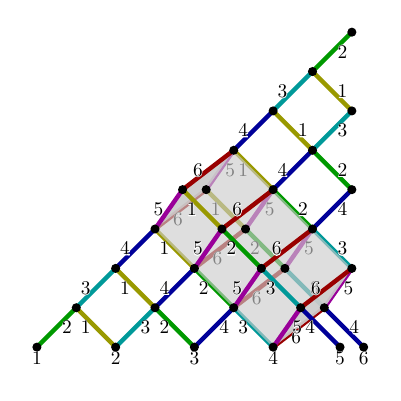
\begin{tikzpicture}
	\hasse{D}{6}%
	\forAllPositiveRootsInHasseDiagram{\foo}%
\end{tikzpicture}
\end{Verbatim}
\begingroup
\tikzset{/Lie Hasse diagram/edge quotes/.style={opacity=0},
	/Dynkin diagram/edge length=1.5cm}
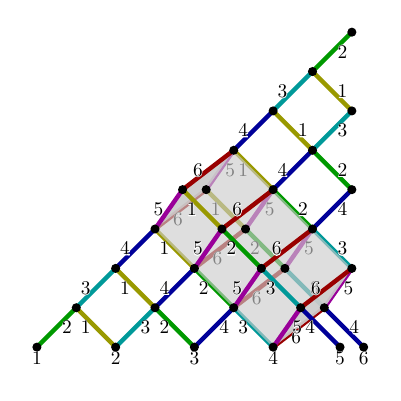
\begin{tikzpicture}
	\hasse{D}{6}%
	\forAllPositiveRootsInHasseDiagram{\foo}%
\end{tikzpicture}

If you put this into the \verb!for all roots! option, it executes on its own:
\begin{Verbatim}
\tikzset{/Lie Hasse diagram/for all roots/.code 2 args={\foo{#1}{#2}}}
\hasseDiagrams{C4;D4}
\end{Verbatim}
\begingroup
\tikzset{/Lie Hasse diagram/for all roots/.code 2 args={\foo{#1}{#2}}}
\hasseDiagrams{C4;D4}
\endgroup
\endgroup

\section{Three dimensional effect}
We draw the \(D,E,F\) Hasse diagrams, following Ringel \cite{Ringel:2013}, as an arrangement of cubes.
Nutma \cite{Nutma:2010} draws the Hasse diagrams using a more elementary approach, but including also the affine Kac--Moody algebras. 
Opposite sides of any square have the same edge label, by commutativity of addition.
Hence we don't need to see every edge perfectly.
The three dimensional effect is the default: 
\begin{Verbatim}
\hasse{D}{4}\hasse{E}{6}
\end{Verbatim}
\begin{center}
\hasse{D}{4}\hasse{E}{6}
\end{center}
We can turn it off:
\begin{Verbatim}
\hasse[three D=false]{D}{4}
\hasse[three D=false]{E}{6}
\end{Verbatim}
\begin{center}
\hasse[three D=false]{D}{4}
\hasse[three D=false]{E}{6}
\end{center}
or globally with \verb!\tikzset{/Lie Hasse diagram/three D=false}!.

The astute reader will perhaps notice that the three dimensional effect is not realistic.
To be Hasse diagrams, the roots have to line up horizontally by grade.
This is inconsistent with three dimensional projection of our cubes.
We have also tried to use only a small number of layers in the three dimensional geometry, so the images are not perfect, but easy enough to read.

We can change the \verb!z shift! to slant the three dimensional images to the right:
\begingroup
\begin{Verbatim}
\hasse[z shift=.1]F4\hasse[z shift=.2]F4\hasse[z shift=.3]F4\hasse[z shift=.4]F4
\end{Verbatim}
\hasse[z shift=.1]F4\hasse[z shift=.2]F4\hasse[z shift=.3]F4\hasse[z shift=.4]F4
\endgroup

We only use three colours and opacities for the faces:
\begin{Verbatim}
	top/.style={black!20,opacity=.4},
	left/.style={black!20,opacity=.9},
	right/.style={black!20,opacity=.6},
\end{Verbatim}
You can change these:
\begin{Verbatim}
\hasse[
	top/.style={red,opacity=.1},
	right/.style={red,opacity=.2},
	left/.style={red,opacity=.4}]E6
\end{Verbatim}
\begin{center}
\hasse[
	top/.style={red,opacity=.1},
	right/.style={red,opacity=.2},
	left/.style={red,opacity=.4}]E6
\end{center}

\section{Label the simple roots}
Ringel \cite{Ringel:2013} labels his edges like
\begin{Verbatim}
\hasseDiagrams{[labels={f,e,d,c,u,b,a}]E7}
\end{Verbatim}
\hasseDiagrams{[labels={f,e,d,c,u,b,a}]E7}

\section{Parabolic subgroups}
This package offers nothing over Ringel's original pictures, except that the user can pick some simple roots whose associated edges are drawn differently.
The chosen simple roots are called \emph{compact}, following terminology from the theory of parabolic subgroups.
We let the reader explore the notation for parabolic subgroups in the Dynkin diagrams package, and use this to declare various roots compact.
\begin{Verbatim}
\tikzset{/Lie Hasse diagram,attach Dynkin diagram=true,three D=false}
\hasseDiagrams{D{**x*x*x*}}
\end{Verbatim}
\begingroup
\tikzset{/Lie Hasse diagram,attach Dynkin diagram=true,three D=false}
\hasseDiagrams{D{**x*x*x*}}
\endgroup
Our motivation comes from trying to identify the invariant vector subbundles of the tangent bundle of a rational homogeneous variety \cite{MathOverflow:123801}.
Such diagrams are often unreadable if we don't turn off the three dimensional graphics.
By default, noncompact root edges are not drawn.
\begingroup
\tikzset{/Lie Hasse diagram,attach Dynkin diagram=true,show name=false,three D=false}
\begin{Verbatim}
\hasseDiagrams{E{*xx*x*}}
\end{Verbatim}
\hasseDiagrams{E{*xx*x*}}
\begin{Verbatim}
\hasseDiagrams{A{x*x*}}
\end{Verbatim}
\hasseDiagrams{A{x*x*}}
\begin{Verbatim}
\hasseDiagrams{[parabolic=113]B8}
\end{Verbatim}
\hasseDiagrams{[parabolic=113]B8}
\begin{Verbatim}
\hasseDiagrams{C{**xx*x**}}
\end{Verbatim}
\hasseDiagrams{C{**xx*x**}}
\newpage
\begin{Verbatim}
\hasseDiagrams{E{*x*x*x**}}
\end{Verbatim}
\hasseDiagrams{E{*x*x*x**}}
\newpage
\begin{Verbatim}
\hasseDiagrams{F{**xx}}
\end{Verbatim}
\hasseDiagrams{F{**xx}}
\begin{Verbatim}
\hasseDiagrams{G{*x}}
\end{Verbatim}
\hasseDiagrams{G{*x}}
\endgroup

\section{Examples}
\begingroup
\tikzset{/Lie Hasse diagram,attach Dynkin diagram=true,show name=true}
\begin{Verbatim}
\hasseDiagrams{A1;A2;A3;A4;A5;A6}
\hasseDiagrams{B3;B4;B5}
\hasseDiagrams{C2;C3;C4}
\hasseDiagrams{C5;C6}
\hasseDiagrams{E6;E7}
\hasseDiagrams{E8}
\hasseDiagrams{F4;G2}
\end{Verbatim}
\hasseDiagrams{A1;A2;A3;A4;A5;A6}
\hasseDiagrams{B3;B4;B5}
\hasseDiagrams{C2;C3;C4}
\hasseDiagrams{C5;C6}
\hasseDiagrams{E6;E7}
\hasseDiagrams{E8}
\hasseDiagrams{F4;G2}
\endgroup 

\section{Black and white}
Publishing in colour on paper can be expensive.
Simple global options:
\begin{Verbatim}
\tikzset{
	background rectangle/.style={
		shade,
		top color=gray!15,
		bottom color=white,
		draw=gray!5,
		very thick,
		rounded corners},
	/Dynkin diagram/text style/.style={black,scale=.75},
	/Lie Hasse diagram,
	edge length=1cm,
	edge/.style={draw=black!50,ultra thick},
	edge quotes/.style={black,auto,inner sep=3pt,scale=.75},
	three D=true,
	show name=true}
\end{Verbatim}
\begingroup
\tikzset{
	background rectangle/.style={
		shade,
		top color=gray!15,
		bottom color=white,
		draw=gray!5,
		very thick,
		rounded corners},
	/Dynkin diagram/text style/.style={black,scale=.75},
	/Lie Hasse diagram,
	edge length=1cm,
	edge/.style={draw=black!50,ultra thick},
	edge quotes/.style={black,auto,inner sep=3pt,scale=.75},
	three D=true,
	show name=true}%
change our examples to
\hasseDiagrams{A1;A2;A3;A4;A5;A6}
\hasseDiagrams{B3;B4;B5}
\hasseDiagrams{C2;C3;C4}
\hasseDiagrams{C5;C6}
\hasseDiagrams{E6;E7}
\hasseDiagrams{E8}
\hasseDiagrams{F4;G2}
\endgroup

\bibliographystyle{amsplain}
\bibliography{lie-hasse}
\end{document}
